\section{Evaluation Results}\label{sec:clientresults}

\begin{table*}[th!]\small
\begin{tabularx}{\textwidth}{|c|c|c|X|}
\hline
\textbf{\S} & \textbf{Figures \& Tables} & \textbf{Data Source} & \textbf{Description} \\
\hline
\ref{sec:controlledexperiments} & Table~\ref{tab:tmobile_rrc_state} & Controlled experiments using \TReport{T-Mobile devices}\Paperonly{carrier C1} & RRC state timers inferred \\
\hline
\ref{sec:controlledexperiments} & Figure~\ref{fig:all_carrier_rrc_delays} & Controlled experiments using \TReport{T-Mobile devices}\Paperonly{carrier C1} & Unexpected high-latency transitions detected; behavior device-dependent \\
\hline
\ref{sec:controlledexperiments} & Table~\ref{tab:extra_tests} & Controlled experiments using \TReport{T-Mobile devices}\Paperonly{carrier C1}  & Impact on higher-layer protocols measured. DNS, TCP handshakes affected by RRC state; HTTP independent\\
\hline 
\ref{sec:qxdm.analysis} & Table~\ref{tab:tmobile_rrc_state} & \emph{QxDM\_{}TCP\_{}Trace} \& \emph{QxDM\_{}UDP\_{}Trace} & RRC state timer validation in QXDM \\
\hline
\ref{sec:qxdm.analysis} & Figure~\ref{fig:udp.rlc.prove}, Figure~\ref{fig:RLC.Loss.Per.RRC.UDPTrace}, Figure~\ref{fig:RLC.Dup.Ack} & \emph{QxDM\_{}TCP\_{}Trace} \& \emph{QxDM\_{}UDP\_{}Trace} & Root cause analysis of unexpected latencies using cross-layer mapping mechanism \\
\hline 
\ref{sec:qxdm.analysis} & Figure~\ref{fig:udp.loss}, Figure~\ref{tab:udp.loss.root.cause} & \emph{QxDM\_{}UDP\_{}Trace} & Analyze root cause of UDP packet loss behavior \\
\hline 
\ref{sec:largescalestudy} & Figure~\ref{fig:timer_cdf} & Public deployment &  Inferred RRC implementations globally; varies by carrier\\
\hline
\ref{sec:largescalestudy} &  Figures~\ref{fig:all_carrier_rrc_delays} and Figure~\ref{fig:loss_compare} & Public deployment & Confirm delays and losses during state transitions a common problem \\
\hline
\ref{sec:largescalestudy} & Figure~\ref{fig:device_compare} & Public deployment & Device-dependence of RRC performance\\
\hline
\end{tabularx}
\ncaption{Summary of key results}
\label{tab:result.summary}
\end{table*}

First, we describe our findings from our client-based RRC inference approach applied to devices applied to devices in controlled experiments, and next describe how we used QxDM-based cross-layer analysis to verify our findings and investigate root causes of our observations, in particular the impact of transient states.  Next, in \S\ref{sec:largescalestudy} we describe the results of the public deployment of our inference tool to examine the representativeness of our findings for RRC states worldwide. Our results are summarized in Table~\ref{tab:result.summary}.  For privacy reasons, we anonymize all data that might identify users when collecting data\Paperonly{, and anonymize the names of all devices and carriers in describing our results}.

%We took two main types of RRC inference-related measurements.  First, we took measurements in a controlled setting, using a set of custom RRC inference tools. There were two main components of these tests that we describe below:  a controlled deployment within T-Mobile of our client-based inference tool on experimental devices, and a set of experiments on local devices requiring QxDM analysis.  Our preliminary tests to develop the RRC inference algorithm were described in \S\ref{sec:stateinferencemethodology} and we do not repeat them here.

%Second, we also deployed a pared-down version of our coarse-grained timer inference tool in order to understand global trends in RRC state machine behavior. The most important difference between that tool and our internal tool is that our internal tool always perform a complete set of tests, whereas the widely-distributed version may take an incomplete set of measurements if there is a loss of cellular connectivity (for example, if the device switches to WiFi.) These tests allow us to understand trends in RRC state implementations and performance around the world, and how they differ by carrier, device model and network technology.We describe the results of these tests in \S\ref{sec:largescalestudy}.


\subsection{Controlled Experiments}\label{sec:controlledexperiments}

We collected three types of data from our controlled experiments: results from a small number of test devices on various carriers, to develop and validate our analysis methodology; \Paperonly{results from a deployment within a large U.S. carrier we call \emph{C1}}\TReport{results from a deployment within T-Mobile}, to measure RRC states and performance characteristics; and results from QxDM traces to validate the \Paperonly{C1}\TReport{T-mobile} results and investigate root causes of the phenomena we detected.  %The results of our first set of tests were confirmed with power monitor measurements as well as through discussions with Carrier C1 to verify our findings.  
We primarily discuss the second two sets of results in this section.

The inference measurements from the \Paperonly{C1}\TReport{T-mobile} deployment are shown in Table~\ref{tab:tmobile_rrc_state}. These timers have changed since being measured in previous work~\cite{3g_rrc}, underscoring the usefulness of a tool that can be used to crowdsource the taking of continuous measurements.   What is of particular interest is the increase in latency when transitioning from DCH to FACH for UMTS. This latency generally lasts from 1 to 2.5s.  A similar pattern was occasionally seen when promoting to DCH, but generally lasts no more than half a second.  Likewise, this delay sometimes occurred in LTE when demoting to RRC\_{}IDLE, although it was only observed in our public deployment. An example of this phenomenon can be seen in Figure~\ref{fig:rtt_raw_data_22}.  This delay is of particular concern because the associated RTTs are often significantly longer even than those in PCH. In some cases, the user derives no benefit from the low-power FACH state at all, as this phenomenon lasts long enough that the expected FACH behavior is never observed.

%Using our internal deployment, we found that the timers and state machines were consistent for devices in several locations across the U.S.  We focused primarily on measuring demotion timers and performance in each RRC state. For LTE, we found a timer of 10s to transition from the high-power to low-power state.  We did not find any transition delays in LTE for our controlled study, likely because of the limited number of devices, as devices in our public study exhibited this behavior. For standard UMTS, we found a 2.5s timer to demote to FACH and another 2.5s timer to demote to PCH, and also detected a period of high latency when demoting from DCH to FACH, lasting from 1 to 2.5s. In other words, in some cases, this phenomena prevented any performance gains from using FACH. There were a small number of devices on an EDGE network, from which we detected two demotion timers demotion timer of 2.5s between the low-power and high-power state, with no intermediate state detected.  A single device on HSDPA had a timer of 2.5s to demote to the low-power state, also with no intermediate state.  % ALL VALUES FINAL

%There is a second RRC state machine deployed in some locations for 3G that we did not detect. 


%Figure~\ref{fig:network_tech_compare} summarizes the difference between UDP RTTs for different RRC states.  We classify DCH and RRC\_{}CONNECTED, for 3G and 4G technologies, as high power; IDLE and RRC\_{}IDLE as low-power, and FACH as medium-power.  The RTT spike when transitioning from DCH to FACH is indicated as ``transition", and for this carrier occured only for UMTS. No error bars are shown for HSDPA since we only have one set of measurements for this technology.  

%In general, performance improves slightly for newer technologies, especially when going from DCH to FACH. Consistent with previous work~\cite{4g_rrc}, improvements in latency between LTE and 3G technologies are not dramatic. It was found in previous work that is mostly bandwidth where LTE benefits, and the largest improvements are in the low-power state for large packets, albeit with a very high variance in our measurements.  It can be seen clearly here that the worst performance (aside from EDGE) is in the transition period between DCH and FACH, and furthermore that the average latency for small packets in FACH is not substantially better than in PCH.

%TODO: higher-level protocols
%TODO: measure latency again


%\begin{figure}[t!]
%\begin{center}
%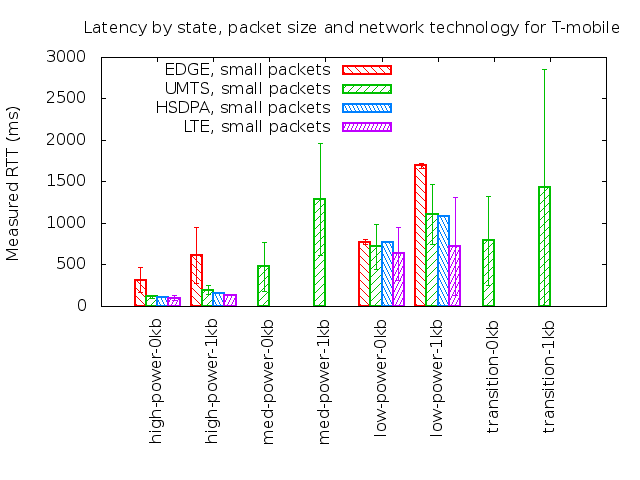
\includegraphics[width=0.45\textwidth]{figs/network_tech_compare.png}
%\end{center}
%\ncaption{Performance of Various Network Technologies for a Single Carrier (T-Mobile)}
%\label{fig:network_tech_compare}
%\end{figure}

We examined the impact of RRC state on several higher-level protocols as well.  We investigated the time to complete a DNS lookup, a TCP handshake, and the loading of a small webpage over HTTP to illustrate the impact of promotion overhead.  For the DNS test, we generated a random, invalid URL, as we found that on some devices the DNS cache could not be flushed.  For TCP, we measured the time to perform a TCP handshake with \url{www.google.com}, and we measured the time to access \url{www.google.com} through HTTP. The results are summarized in Table~\ref{tab:extra_tests}.

In general, there was a very high variance for the data collected in each of the states. TCP handshakes and DNS lookups, like raw UDP packets, appear to be affected by the RRC state of the initial packet sent, in large part because these tests involve few packets.  For HTTP, however, the impact of the starting RRC state was not statistically significant.  This is also unsurprising, as the RRC state only affects the first packet sent.  FACH\_{}TRANSITION appears to have a performance impact, however. RRC state would primarily impact frequent, low-bandwidth transmissions, such as applications that perform periodic polling, as observed in previous work~\cite{aro}. 

\begin{table}[t!]\small
\begin{tabularx}{0.5\textwidth}{|X|X|X|X|X|}
\hline
\textbf{Network Type} & \textbf{DCH/ RRC CONNECTED (s)} & \textbf{FACH (s)} & \textbf{Transition delay?} & \textbf{\# devices observed}\\
\hline \hline
UMTS & 3 & 2 & Yes* & 12 \\
\hline
HSDPA & 3 & None & No & 1 \\
\hline
LTE & 10 & None & No & 3 \\
\hline
EDGE & 2 & None & No & 3 \\
\hline \hline
\multicolumn{5}{|c|}{\textbf{QxDM Ground Truth}} \\
\hline\hline
UMTS & 3.2 & 2.3 & Yes & 2 \\
\hline
\end{tabularx}
* For a subset of devices
\ncaption{Inferred timers for controlled experiments on a major US carrier; ground truth for UMTS from QxDM} 
\label{tab:tmobile_rrc_state}
\end{table}

\begin{table}[t!]\small
\begin{tabularx}{0.5\textwidth}{|X|X|X|X|X|}
\hline
\textbf{Protocol} & \textbf{DCH (ms)} & \textbf{FACH TRANSITION (ms)} & \textbf{FACH (ms)} & \textbf{PCH (ms)} \\
\hline \hline
DNS lookup (UDP)& 449 $\pm$ 881  & 1656 $\pm$ 1157 & 776 $\pm$ 948 & 1209 $\pm$ 1350 \\
\hline
TCP handshake & 229 $\pm$ 191 & 1524 $\pm$ 1371 & 1114 $\pm$ 1096 & 936 $\pm$ 674 \\
\hline
HTTP & 3120 $\pm$ 6465 & 3530 $\pm$ 4905 & 2926 $\pm$ 1609  & 3338 $\pm$ 6031 \\
\hline
\end{tabularx}
\ncaption{Comparison of 3G performance across different RRC states for higher-level protocols. FACH TRANSITION refers to a period of high latency when packets are sent during promotions to FACH due to RLC-layer transient state behavior. Note RRC state dependence of DNS and TCP in particular.}
\label{tab:extra_tests}
\end{table}

%\begin{figure}
%\begin{center}
%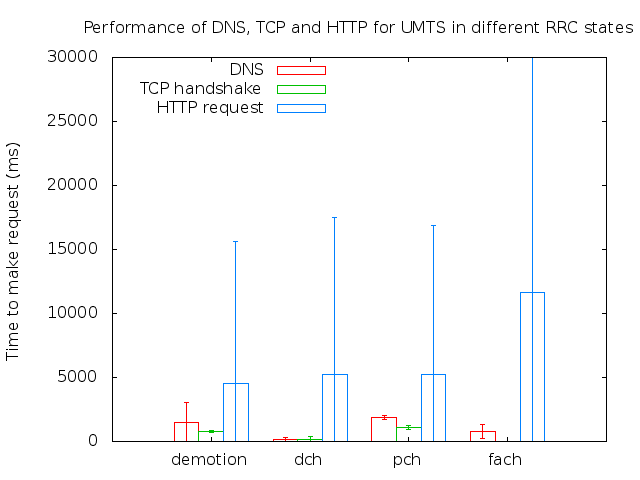
\includegraphics[width=0.45\textwidth]{figs/extra_tests.png}
%\end{center}
%\ncaption{Impact of RRC state on non-UDP protocols}
%\label{fig:extra_tests}
%\end{figure}

\subsubsection{Cross-Layer Root-Cause Analysis with QxDM}\label{sec:qxdm.analysis}
% TODO: include the infered timer part here
We first validate the inferred RRC timers using the method described in \S\ref{sec:exp.setup}. The time difference between the last IP packet and the associated RBR message is around 3.2 seconds. Similarly, the PCH demotion timer is approximately 2.3 seconds, based on the time difference between the last IP packet in FACH and the associated PCR message. The first timer result matches the one in Table~\ref{tab:tmobile_rrc_state} exactly, rounding to the nearest half-second (as that is the granularity at which the measurements were taken). The second timer matches closely as well.

Next, we examine the root cause of the unexpected latencies when transitioning between RRC states. We make use of data from \emph{QxDM\_{}UDP\_{}Trace} and \emph{QxDM\_{}TCP\_{}Trace}.
%, and in \S\ref{sec:eval} we propose an approach to avoid these unexpected latencies.  We also identify the prevalence and root causes of UDP packet losses. In this section, 
Making use of the terminology defined in \S\ref{sec:background}, we examine each of the \emph{transient states} at the RLC layer to understand the root causes of this behavior.  Based on our measurements of the FACH and PCH promotion times, we determine that FACH\_{}PROMOTE covers the time period of 0.92 seconds before promotion to DCH occurs in \emph{QxDM\_{}UDP\_{}Trace} and \emph{QxDM\_{}TCP\_{}Trace}. Similarly, PCH\_{}PROMOTE covers the time period of 0.21 seconds before FACH promotion occurs as defined in Table~\ref{tab:terminology}.

%We identify the root cause of unexpected latencies by making use of results from a set of QxDM measurements that we will refer to as \emph{QxDM\_{}Trace}.  We propose in \S\ref{sec:eval} an approach to avoid these unexpected latencies.  Next, we use \emph{QxDM\_{}Trace} to identify the prevalence and root causes of UDP packet losses.  

%\S~\ref{sec:root.cause.analysis} identifies the root cause of latency by results from both emph{QxDM\_{}Trace}, and propose RLC Fast retransmission mechanism to reduce the RLC delay. \S~\ref{sec:udp.loss.analysis} is a case study of utilizing the cross-layer mapping and retransmission calculation technique to identify the root cause of the UDP packet loss.
%\subsection{Cross-Layer Analysis with QxDM}\label{sec:qxdm.analysis}
%\S~ref{sec:rrc.term} defines and highlights subset of FACH state so that we could have fine grained understanding the abnormal latency issue. \S~\ref{sec:root.cause.analysis} identifies the root cause of latency by results from both emph{QxDM\_{}Trace}, and propose RLC Fast retransmission mechanism to reduce the RLC delay. \S~\ref{sec:udp.loss.analysis} is a case study of utilizing the cross-layer mapping and retransmission calculation technique to identify the root cause of the UDP packet loss.

%However, as at the RLC layer we can observe various phenomena that are not detectable at higher layers, we will start by defining some terminology. Because the the promotion period for PCH and FACH differs from their initial period due to additional signaling overhead, we want to distinguish between a RRC state with and without involving transitions. Since we focus on the initial period of data transmission, the RRC state promotion is more meaningful than state demotion, which is the end of whole data transmission period. So RRC state promotion is our preliminary concern for this project. We break down the normal FACH into an initial FACH state and FACH to DCH promotion state, named as FACH\_{}INIT and FACH\_{}PROMOTE specifically. Similarly, PCH was divided into PCH\_{}INIT and PCH\_{}PROMOTE.

%Since the FACH promotion timer is on average 0.92 seconds and PCH promotion state is on average 0.21 seconds, we consider the time
%define the FACH\_{}PROMOTE state as the time slot of counting back 0.92 seconds from the point of promoting to DCH. For the same reason, PCH\_{}PROMOTE state describes the time slot of counting back 0.21 seconds from the point of promoting to FACH.

%\subsubsection{Root Cause of Latency}\label{sec:root.cause.analysis}
% explain why we want to calculate RLC layer retransmission and how to calculate

To demonstrate the strong correlation between data link layer retransmissions and higher layer latencies, we calculate the RLC layer retransmission ratio for each inter-packet time interval using the methodology described in \S\ref{sec:rlc.retx.cal}. We insert the inter-packet time for the test performed in the packet payload for data in the \emph{QxDM\_{}UDP\_{}Trace}, so we can directly correlate the RLC PDUs with the associated inter-packet timing after we apply the cross-layer mapping algorithm from \S\ref{sec:cross.layer.algo}. In Figure~\ref{fig:rlc.retx.gap} the high retransmission ration in FACH can be seen, which matches the latency behavior in Figure~\ref{fig:udp.rtt.gap}. The similar patterns imply that the root cause of the FACH latency issue resides in the data link layer.

\begin{figure}[t!]
\centering
%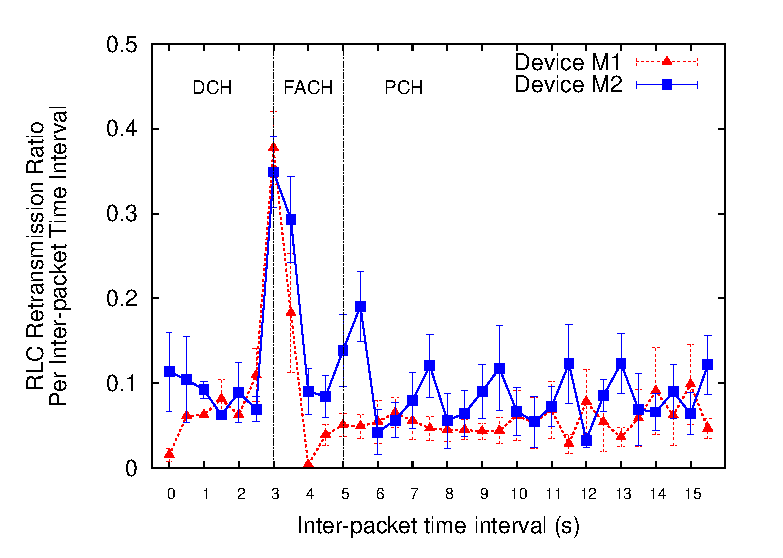
\includegraphics[width=0.5\textwidth]{figs/rlc_retx_gap.eps}
%\begin{subfigure}
%\centering
%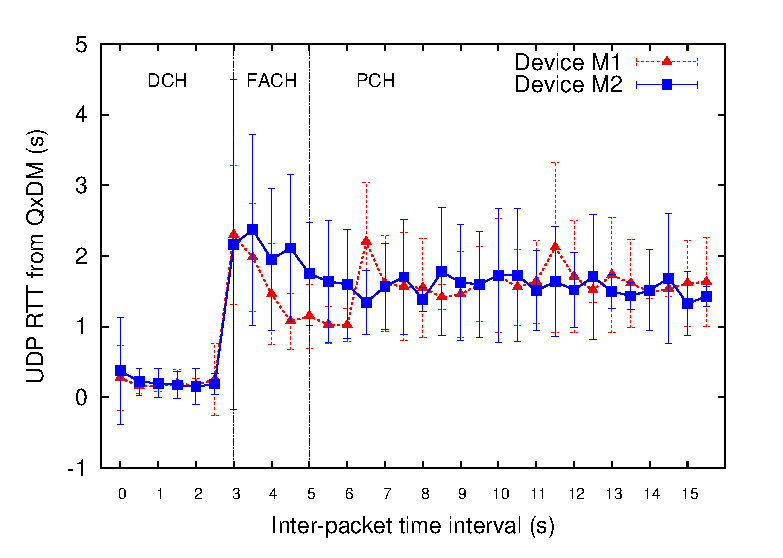
\includegraphics[width=0.5\textwidth]{figs/udp_rtt_gap.eps}
%\label{fig:udp.rtt.gap}
%\end{subfigure}%
%\begin{subfigure}{0.5\textwidth}
%\centering
%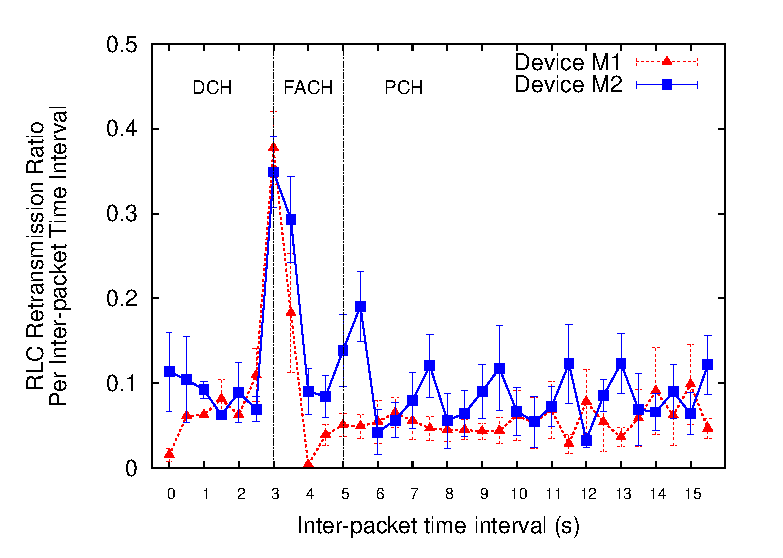
\includegraphics[width=0.5\textwidth]{figs/rlc_retx_gap.eps}
%\label{fig:rlc.retx.gap}
%\end{subfigure}
\subfigure[UDP RTT Result]{\label{fig:udp.rtt.gap}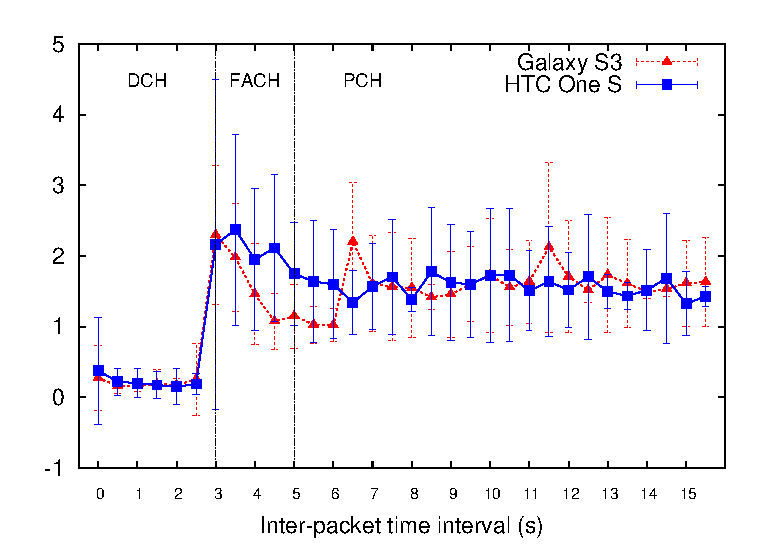
\includegraphics[width=0.5\textwidth]{figs_nonanony/udp_rtt_gap.eps}}\\%
\vspace{-3.0ex}
\subfigure[RLC Retransmission Result]{\label{fig:rlc.retx.gap}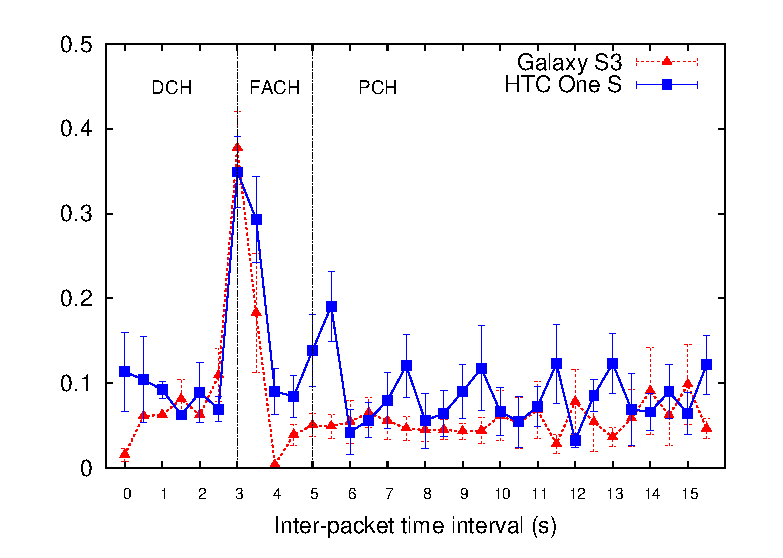
\includegraphics[width=0.5\textwidth]{figs_nonanony/rlc_retx_gap.eps}}%
\ncaption{RLC layer retransmission ratio has a strong correlation with the delay over FACH state. Measurements on 1 KB packets.}
\label{fig:udp.rlc.prove}	
\end{figure}

There are two possible RLC retransmission behaviors that lead to delays at the transport layer. First, retransmission may be necessary due to noisy channel conditions during FACH. Based on the \emph{QxDM\_{}UDP\_{}Trace} and the \emph{QxDM\_{}TCP\_{}Trace}, we can see that RLC retransmission ratios are particularly high during FACH.  A possible solution to this problem is for the application to batch data transmissions to reduce the frequency of RRC state promotions, a solution that has been shown to be beneficial in eliminating other transmission-related delays~\cite{3g_rrc}.  Second, retransmissions can become unnecessarily delayed due to a slow response to the PDU loss signal (i.e., duplicated ACKs). In particular, this can effect TCP transmissions, as the relationship between TCP retransmissions and RLC retransmissions leads to delays.  We propose a solution to address this latter problem in \S\ref{sec:eval}.

%a strong correlation between RLC retransmission ratio and FACH state as an evidence. One possible solution is that application could batch the data transmission to reduce the RRC state promotion frequency~\cite{3g_rrc}. The second one is the retransmission get unnecessary delayed caused by the lagging response to the PDU loss signal. We also observe it from \emph{QxDM\_{}Trace} when we studied the relationship between TCP retransmission and RLC retransmission. We will also provide a improved RLC mechanism to avoid the unnecessary delay later.

% UDP trace analysis

Using the RLC retransmission calculation methodology described in \S\ref{sec:rlc.retx.cal}, we calculate the RLC transmission ratio for each transient state. We show these results in Figure~\ref{fig:RLC.Loss.Per.RRC.UDPTrace}. The retransmission ratios are particularly high in FACH\_{}INIT and FACH\_{}PROMOTE. For the \Paperonly{M2}\TReport{HTC} device, the ratio is especially high during FACH\_{}INIT. These observations are consistent with the abnormal delays we observed when transitioning from DCH to FACH at the UDP layer. The higher loss rates for the device made by \Paperonly{M2}\TReport{HTC} are consistent with the differences between devices found in the public study in \S\ref{sec:largescalestudy}. A possible explanation is the difference in hardware used. \Paperonly{The M1 and M2 devices use two different generations of chipsets, and the newer one  supports a larger range of network types}\TReport{The HTC device uses Snapdragon S3 MSM8260, while the Galaxy S3 contains the next-generation Snapdragon S4 MSM8960 and supports a larger range of network types}~\cite{snapdragon}. This chipset dependency might also explain why this phenomenon was not observed in earlier work, on older devices, which likely used yet another chipset. In our public study we found that there are a number of chipsets from various companies that exhibit this behavior. However, a detailed examination of hardware differences is out of the scope of the paper.

%HTC device uses Snapdragon S3 MSM8260, while the Galaxy S3 contains the next-generation Snapdragon S4 MSM8960 and supports a larger range of network types~\cite{snapdragon}. This 

%Analyzing the \emph{QxDM\_{}Trace} based on the RLC retransmission calculation methodology, we calculate the RLC retransmission ratio per RRC state in Figure~\ref{fig:RLC.Loss.Per.RRC.UDPTrace}. As we can see, the RLC retransmission among FACH and FACH\_{}PROMOTE in total are \textit{46.63\%} for HTC One S device with standard deviation of \textit{4.28\%}, and \textit{14.23\%} for Galaxy S3 devices with standard deviation of \textit{0.66\%}. It strongly suggested the significant delay over the FACH\_{}INIT and FACH\_{}PROMOTE states, which indicates the higher chance of RLC retransmission in a resource shared and noisy channel during FACH state. The observation is consistent with the abnormal delays during initial FACH state as we could also observe radio bearer configuration signaling and other system signaling exchange between the handset and the base station. We also observe that the HTC device has a higher loss rate than that of Galaxy S3. One possible explanation for device dependent behavior is that the difference in hardware module. The HTC One S was produced over Snapdragon S3 MSM8260, while the Galaxy S3 contains Snapdragon S4 MSM8960, which is the next generation of the one for HTC One S. The wireless radio techniques for Snapdragon S4 has support for larger range of network types~\cite{snapdragon}. The detailed discussion about the hardware differences is out of the scope of this paper.

% RLC Loss ratio per RRC state
\begin{figure}[t!]
\centering
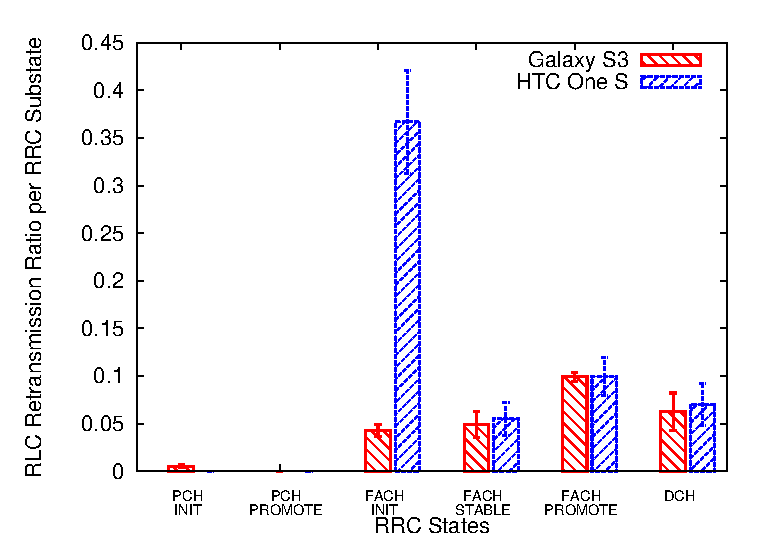
\includegraphics[width=0.5\textwidth]{figs_nonanony/rlc_retx_udp.eps}
\ncaption{The significant RLC retransmission ratio over the stable FACH state and FACH promotion state is consistent with higher-layer measurements and suggests that FACH\_{}INIT has a significant impact on the FACH transition delay.}
\label{fig:RLC.Loss.Per.RRC.UDPTrace}
\end{figure}

%TCP Trace Analysis
We also examined performance in TCP. A TCP \textit{retransmission timeout} (RTO) can cause a RTT delay as the congestion window size decreases and the device falls back to the slow start phase~\cite{tcp.rto}. We use our mapping algorithm to correlate TCP retransmission behavior with RLC retransmissions. We found that the current RLC protocol responds sluggishly to the duplicate ACKs that signal that a PDU has been lost (see Figure~\ref{fig:RLC.Dup.Ack}). This leads to a TCP RTO which introduces more latency in the transport layer.  

According to the 3GPP RLC specification, the sender only retransmits the PDU once it receives a STATUS LIST (i.e., non-acknowledged) control PDU from the receiver, ignoring duplicate ACKs~\cite{spec-3G-RLC}. These duplicate ACKs are strong hints for PDU losses. If the lost RLC PDUs were to be transmitted after 0.5s rather than 2.8s, then the TCP RTO could be avoided, reducing latency by more than 2.3s. We propose a RLC \textit{Fast Re-Tx} mechanism, where unacknowledged PDUs are retransmitted once three duplicate RLC PDU ACKs are received by the sender. The resulting faster reaction to lost signals would reduce both RLC latency and latency in the transport layer. We evaluate this mechanism in \S\ref{sec:eval}

%The TCP retransmission timeout (RTO) could cause apparent round trip delay due to congestion window drop by half and restarting the data transmission from the slow start phase~\cite{tcp.rto}. From the \emph{QxDM\_{}Trace}, we correlate the TCP retransmission behavior with the RLC retransmission through our mapping algorithm. By capturing the root cause of the TCP RTO, we found that current RLC protocol has a sluggish response to the PDU lost sigals -- the duplicate ACKs, in Figure~\ref{fig:RLC.Dup.Ack}. The delayed RLC retransmission PDUs leads TCP RTO, which further introduces latency in the transport layer. In 3GPP RLC specification, the sender only retransmits the PDU once it receives the STATUS LIST (or non-acknowledged) control PDU from the receiver, but ignores to duplicate ACKs, which is a strong hint for PDU loss~\cite{spec-3G-RLC}. If we could bring the group of retransmitted RLC PDUs from 2.8 s to 0.5 s, then we could avoid TCP RTO, reducing the latency more than 2.3 s. Therefore, we propose a RLC \textit{Fast Re-Tx} mechanism, which will retransmit the unacknowledged PDUs once the sender receives three duplicate RLC PDU ACKs. The faster reaction to loss signals could reduce RLC layer latency and further reduce the latency in transport layer.

% explain the root cause of the longer delay analysis
\begin{figure}[t!]
\centering
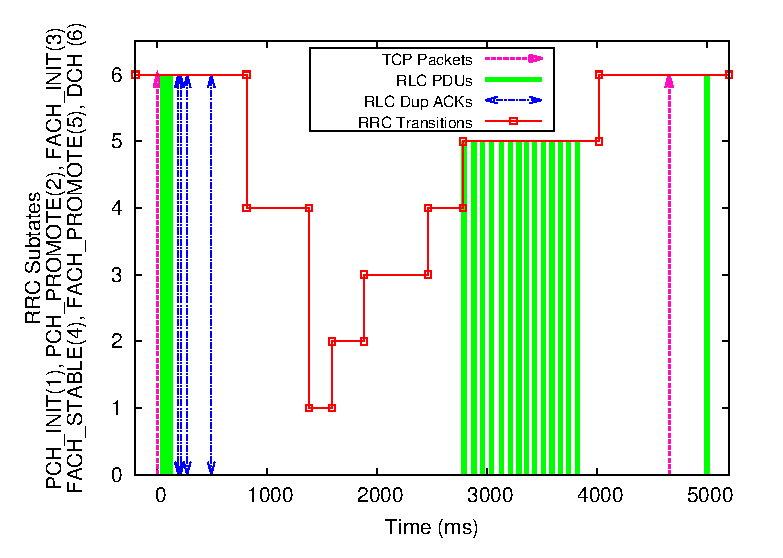
\includegraphics[width=0.5\textwidth]{figs/rlc_dup_ack.eps}
%\ncaption{Two Latency Causes: short DCH demotion timer and lagging response to the PDU lost signal}
\ncaption{TCP RTO is caused by delays in RLC PDU retransmission. Duplicate ACKs suggest a PDU has been lost. By responding to this probable loss in a timely manner, RLC transmission latency can be reduced and sometimes TCP RTOs can even be avoided.}
\label{fig:RLC.Dup.Ack}
\end{figure}

% UDP loss analysis
%\subsubsection{Root Cause of Packet Loss}\label{sec:udp.loss.analysis}
Finally, we examine UDP losses in each RRC state and identify root causes of these losses.  We label each packet with a unique ``sequence number" to map UDP packets sent from the client to the server-side tcpdump trace --- a loss occurs when a packet never appears at the server.  We consider the RRC state or RLC-layer transient state associated with each packet to be the state when the packet is sent, as defined in Table~\ref{tab:terminology}.  Packet loss ratios are the ratios between the number of packets lost from each state and those sent.  As can be seen in Figure~\ref{fig:udp.loss}, these losses are highly device-dependent as well, with \Paperonly{the M2 device} \TReport{the HTC device} having a higher loss ratio in DCH and FACH, and the \Paperonly{M1}\TReport{Samsung} device being more lossy in PCH.  As devices perform most transmissions in DCH and FACH, the \TReport{Samsung}\Paperonly{M1} device is less lossy overall.

%UDP protocol doesn't guarantee the data package delivery, because the sender doesn't receive feedback from the receiver. We are interested in understanding the UDP loss behaviors over each RRC state, and also identify the root cause of UDP packet loss. As we instrument a unique "sequence number" for every UDP packet in \emph{QxDM\_{}TRACE}, we are able to apply the one-to-one mapping of UDP packet from client side \emph{QxDM\_{}TRACE} to the server side tcpdump trace. Each packet loss is considered as an packet appeared on the client side, but not on the server side. The RRC state of a packet means the state when it was transmitted. The packet loss ratio per RRC state is calculated as the number of packets get lost over that state divided by the total number of packets over that state. In Figure~\ref{fig:udp.loss}, the loss ratio really depends on the devices. HTC One S has a higher loss ratio over, DCH, and FACH state. While Samsung Galaxy S3 is more lossy over the PCH state. As the device is generally stay in DCH and FACH state, the Galaxy S3 will be less loss than the HTC device.

% UDP Loss Ratio plot
\begin{figure}[t!]
\centering
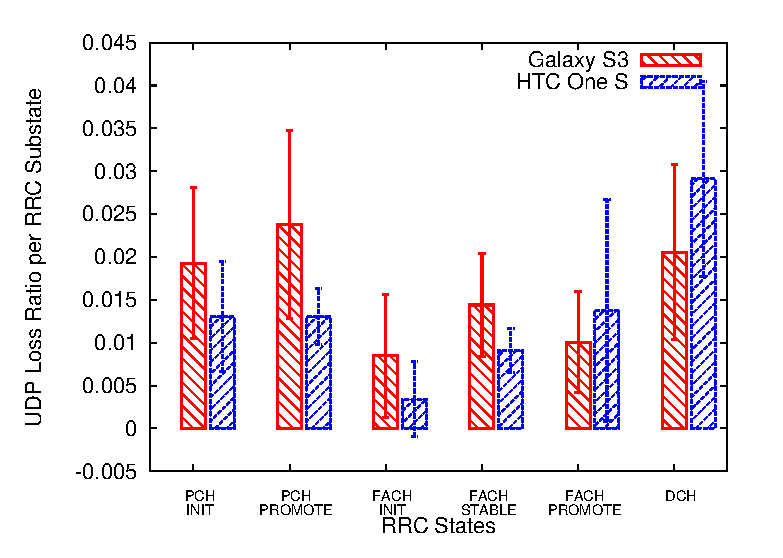
\includegraphics[width=0.5\textwidth]{figs_nonanony/udp_loss.eps}
\ncaption{UDP loss dependence on the device and on RRC transition states}
\label{fig:udp.loss}
\vspace{1ex}
\end{figure}

To identify the root cause of these UDP losses, we use the cross-layer mapping algorithm to understand RLC-layer transient state behavior.  We wish to understand if the UDP packets are getting lost over the OTA link or the wired channel as defined in \S\ref{sec:background}. Since QxDM only captures the data transmission in UTRAN, SDU losses not found in QxDM traces are lost over the wired channel. According to the 3GPP specification~\cite{spec-3G-RLC}, RLC PDUs are lost between the handset and the Node-B due either to senders retransmitting the PDUs more times than a pre-defined limit or due to the sender being reset by the receiver.  After mapping each UDP PDU to the corresponding RLC PDU, we check if the sender received a reset control PDU from the receiver or if the number of retransmitted PDUs exceeds a predefined limit.  If neither case applies, we know that the the UDP packet was lost over the internet.  Most UDP packets are lost over the wired channel, as can be seen in Figure~\ref{tab:udp.loss.root.cause}. This is due to the RLC layer ARQ (Automatic Repeat reQuest) mechanism that limits losses in the RLC layer.

%The UMTS network consists of the mobile devices, the \textit{UMTS Terrestrial Radio Access Network} (UTRAN), and the \textit{Core Network} (CN)

%To identify the root cause of the UDP loss, we apply the cross-layer mapping algorithm, and analyze the RLC layer behaviors. We are interested in whether the UDP packets get lost in the cellular network or in the internet. Based on 3GPP specificaiton~\cite{spec-3G-RLC}, RLC PDUs will be lost in between the handset and the Node-B, because either the sender retransmit the PDU more than a pre-defined limit or the sender was reset by the receiver. After map each UDP packet with a corresponding RLC PDUs, we will check whether the sender received a reset control PDU from the receiver, or the number of retransmitted PDU exceeding the pre-defined limit. The rest of the cases would count as the UDP lost over the internet. In Figure~\ref{fig:udp.loss.root.cause}, most of the UDP packets are lost over the internet, which is primarily because the RLC layer ARQ (Automatic Repeat reQuest) mechanism in the RLC layer. 

% UDP Loss Root Cause
%\begin{figure}[t!]
%\centering
%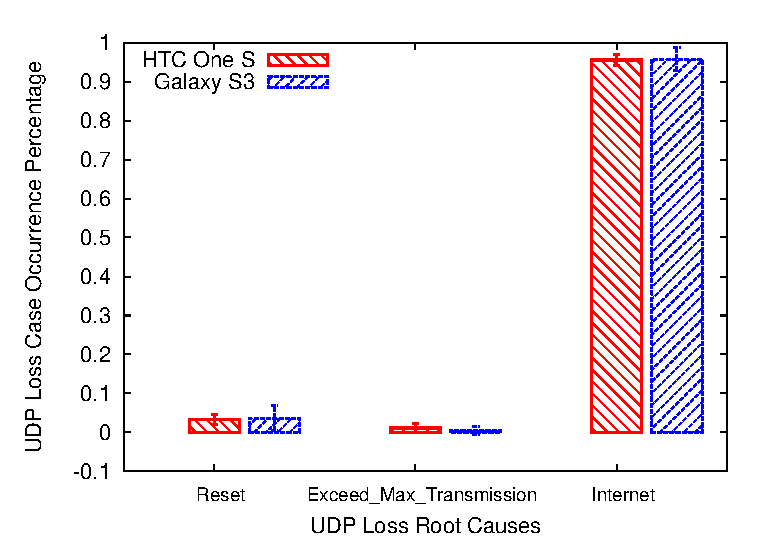
\includegraphics[width=0.5\textwidth]{figs/udp_loss_root_cause.eps}
%\ncaption{The major loss cause of UDP packets comes from internet, but not in the cellular network}
%\label{fig:udp.loss.root.cause}
%\end{figure}

\begin{table}\small
\begin{tabularx}{0.5\textwidth}{|X|X|X|X|}
	\hline
	& \multicolumn{2}{|c|}{\textbf{OTA (\%)}} & \multirow{2}{*}{\textbf{\vbox{Wired (\%)}}} \\ \cline{2-3}
	& \textbf{Reset} & \textbf{Exceed Limit} & \\
	\hline\hline
	\Paperonly{Device M1}\TReport{Samsung SIII} & 3.67$\pm$3.14 & 0.57$\pm$1.01 & 95.77$\pm$3.01 \\
	\hline
	\Paperonly{Device M2}\TReport{HTC One} & 3.32$\pm$1.31 & 1.17$\pm$1.16 & 95.56$\pm$1.37 \\
	\hline
\end{tabularx}
\ncaption{Most UDP packet losses happen in the wired network, not the OTA (or wireless) channel.}
\label{tab:udp.loss.root.cause}
\end{table}

\subsection{Public Deployment of the Inference Tool}\label{sec:largescalestudy}

To get a broader and more representative set of data, we integrated the coarse-grained RTT measurement functionality into Mobiperf~\cite{mobiperf}, an existing network performance measurement application. 
We did not collect data on the impact of RRC state on higher-level protocols, however.


130 devices on 41 carriers in 25 countries have installed the test, based on hashed phone identifiers (to preserve user anonymity). However, we only have complete data on 27 devices, covering 9 countries, 16 carriers and 20 distinct device models from 6 manufacturers.  

%\begin{TReports}
% However, there are two subsets of this data set we exclude.  First, a number of devices (48 in total) never completed sufficient tests.  
%\end{TReports}
We excluded devices with less than three tests run in order to ensure we could effectively filter noise.
\begin{TReports} 
Second, a number of devices never uploaded accurate data on the network technology used --- either because they never updated from the original application version that did not collect this data, or because their device always returns the value "UNKNOWN". We exclude these devices from any findings that require knowing the specific network technology.   We therefore focus on 27 devices with complete data in this section --- these cover 9 countries, 16 carriers and 20 distinct device models from six manufacturers.  

\end{TReports}
%such as the US, Germany, the UAE, Indonesia and China.  Phone identifiers were hashed to preserve user anonymity.  Because of the incomplete data provided by devices in the public test, N devices never uploaded sufficient data to perform the RRC inference task.  N devices had their RRC model flagged as ``anomalous" and after a manual inspection were disregarded due to having insufficient data.
%TODO fill in numbers

In this section, as we are observing higher-level behavior, we do not discuss the transient states directly.  Instead, we refer to the behavior caused by delays during transient states, resulting in UDP-layer delays when sending packets during the transient states associated with a state demotion, as FACH\_{}TRANSITION or LTE\_{}TRANSITION.  The former refers to delays when demoting to FACH, and the latter to delays when demoting to RRC\_{}IDLE.

First, we examine the inferred RRC states for the devices for which data has been collected and examine how these states vary across carriers.  For LTE, we have data from two carriers, both within the U.S.  Both have $T_{Tail}$ timers of 10 seconds.  Some devices exhibited a spike in latency when transitioning between states. There appears to be some device dependency for this effect under LTE as well. A comparison of the latencies and packet losses for two different devices using the same carrier and the same RRC state transition timers can be seen in Figure~\ref{fig:device_compare}. 

The UMTS timers are more varied, and we have more data on a wider range of carriers than for LTE.  The timers are summarized in Figure~\ref{fig:timer_cdf}. Each distinct RRC state machine for a carrier is counted only once regardless of the number of devices collecting data.  Timers are generally closer to 3 seconds when FACH is used and 7 seconds when it is not.  We do not in general have enough data to compare carriers across devices or locations, but when we do, state machine timers are consistent within one second. However, we found that one carrier which uses two different UMTS versions in two different locations has two different sets of timers.  We found that  devices usually enter FACH both during demotion and promotion, or not at all, with one exception where the device promotes directly to DCH but enters FACH during demotion.  


Substantial delays when demoting from DCH to FACH were common. It is less immediately clear that this is device-dependent behavior, though, for two reasons.  First, there are more carriers in this dataset but few devices per carrier, so comparing different devices with the same carrier is often not possible. We did observe for one carrier\TReport{, Verizon,} that not all devices exhibited this behavior, however.  Secondly, there were two cases where, for a specific model of phone, some devices exhibited this behavior and some did not. After some investigation, it seems that different chipsets are used in different markets for the same model of phone, which might explain this discrepancy.  We also determined that several different chipsets from several different manufacturers exhibit this behavior, so the problem is not due to a single poor implementation. However, without more information about each device we cannot be confident in our claim that this is entirely device-specific behavior.

%As can be seen in Figure~\ref{fig:timer_cdf}, certain timers are particularly common. There are a limited number of different RRC state machines that seem to be implemented in practice, even accross very different carriers, and this is especially true for LTE.  Timers of 6-7 seconds for LTE seem to be most common, although in the US timers of 10 seconds were frequently observed. For 3G, there is far more variation, but usually devices fall back to FACH within 2.5 to 4.5 seconds.  FACH can last from 3-5 seconds, with lower values being far more common.


%For most carriers, we have only a small number of devices per carrier, and so it is difficult to determine if the RRC state machine for a specific carrier varies by device or location.  However, for several major US carriers we had a number of different users accross the country.  For example, for AT\&T, we collected data from users in Michigan, California, Pensylvania, and Florida.  The inferred timers for each network technology are almost always consistent accross these geographic regions, within half a second.  The one exception is Verizon ---  we observed two different LTE timers in two different geographic locations with the same model of phone.  

%UMTS allows variation both in the timers between states and in the states available.  As was shown in previous work, some carriers will skip the FACH state either when promoting or demoting\cite{3g_rrc}. We found five distinct 3G RRC state machines that always pass through FACH in both directions, and six that do not enter FACH when promoting from IDLE.  Four additional carriers had the FACH state entirely obscured by the FACH\_{}TRANSITION effect. In those cases it is unclear if FACH is ever entered, but users would not benefit from FACH. Additionally, ten devices did not upload carrier information. Eight entered FACH in both directions, and two did not enter FACH during state promotion.  Most carriers within the US have state machines that enter FACH in both directions, aside from Verizon which exhibited both patterns.  No other RRC state machine patterns were observed.

%, specifically, allows more variation in how it is implemented. As was shown in previous work, some carriers will, upon recieving a packet in IDLE, go directly to DCH regardless of the size of the packet, whereas others might first pass through FACH~\cite{3g_rrc}.  In our survey of carriers, we found five distinct RRC state machines that always pass through FACH whether promoting or demoting, and six that do not enter FACH when promoting from IDLE.  There were four additional RRC state machines where data was sufficiently noisy that a significant number of measurements taken were ambiguous; three of these had the majority of their measurements consistent with entering FACH in both scenarios.  Additionally, eight devices which lacked carrier information entered FACH in both directions, and two did not enter FACH when promoting.

%Single-directional FACH state machines were most common outside of the US; additionally, Verizon exhibited both patterns on different devices.  We did not observe any other RRC state machine patterns. 




\begin{figure}[t!]
\begin{center}
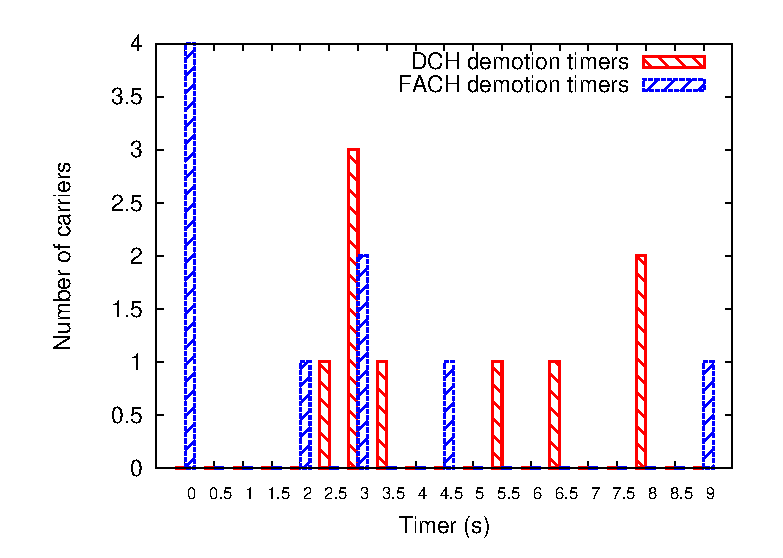
\includegraphics[width=0.45\textwidth]{figs/timer_cdf.eps}
\end{center}
\ncaption{Distribution of RRC 3G timers, for nine UMTS RRC state machines. Note cluster around 2-3.5s.}
\label{fig:timer_cdf}
\end{figure}

\begin{figure}[t!]
\begin{center}
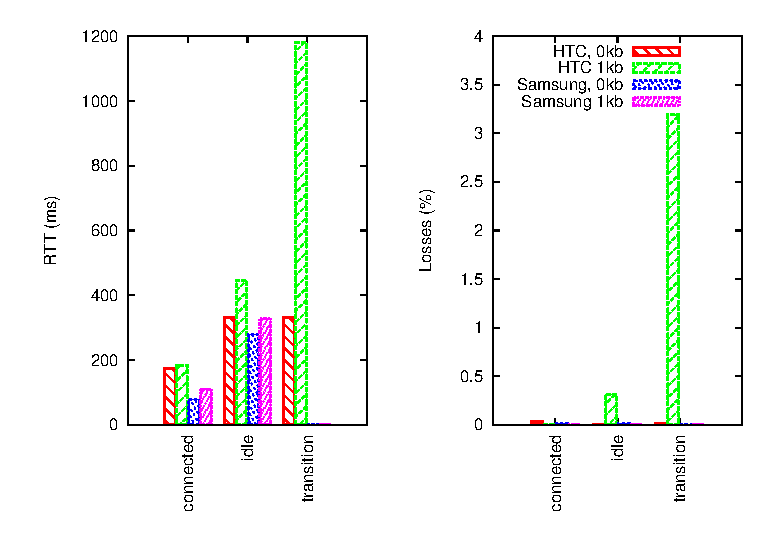
\includegraphics[width=0.5\textwidth]{figs/device_compare.eps}
\end{center}
\ncaption{RTTs and loss rates for two device models on the same LTE network, based on 39 tests for \Paperonly{M1} \TReport{the Samsung SIII} and 94 for \Paperonly{M2}\TReport{ the HTC One}.  Note that only the \TReport{HTC} device \Paperonly{M2} exhibits an additional delay around state demotion. The ``Transition" data is during a period of high latency when sending data around a demotion to RRC\_{}IDLE.}
%\ncaption{RTTs and loss rates for an HTC One and Samsung S3 device on the same LTE network.  Note that only the HTC device exhibits an additional delay around state demotion.}
\label{fig:device_compare}
\end{figure}
We also examined the performance characteristics associated with different RRC states. As most of our data was for LTE or UMTS, we focus on these two technologies. For UMTS, we collected data from 12 devices. Between 16 and 143 tests were run per device (with an average of 70 tests run). We excluded a large number of devices with less than three tests each --- the distribution of measurements per device is very irregular. For LTE, we used 9 devices with an average of 34 tests each, ranging from 4 to 110 tests.

We first  examined the average promotion delays associated with different RRC states, shown in Figure~\ref{fig:all_carrier_rrc_delays}. These are calculated based on the difference in RTT between the highest-power, lowest-latency state and every other RRC state. We see that the pattern we observed for the \Paperonly{Carrier C1}\TReport{controlled T-mobile} dataset holds here as well. Furthermore, LTE generally performs better than 3G.  It can also be seen here that latencies when transitioning between DCH and FACH are quite substantial, and often higher than in PCH.

\begin{figure}[t!]
\begin{center}
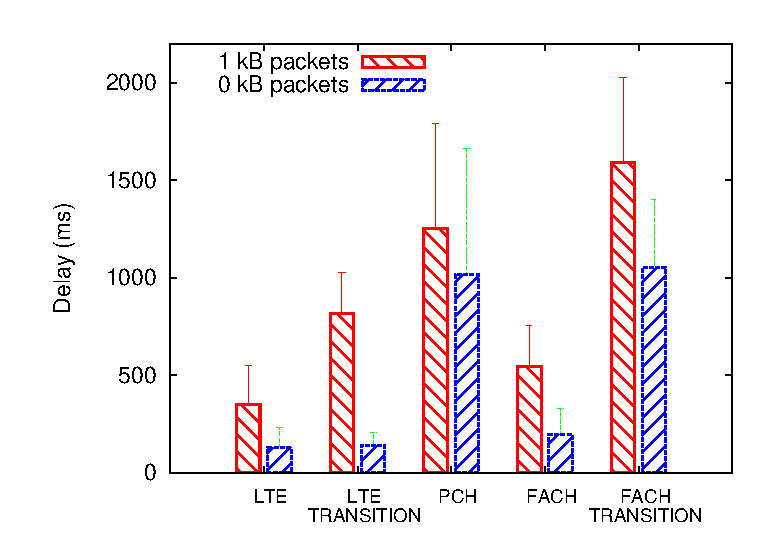
\includegraphics[width=0.45\textwidth]{figs/all_carrier_rrc_delays.eps}
\end{center}
\ncaption{Promotion delays for each state for all carriers surveyed, calculated by subtracting the RTT in the highest-power state from the RTTs in states where promotions are required.  The anomalous behavior FACH\_{}TRANSITION and LTE\_{}TRANSITION, when it occurs, results in significant delays.}
\label{fig:all_carrier_rrc_delays}
\end{figure}

We also examined trends in packet loss in different RRC states for these carriers, as shown in Figure~\ref{fig:loss_compare}, again comparing 3G and LTE.  Unsurprisingly, losses were generally low in high-power states (DCH or RRC\_{}CONNECTED) and are high in low-power states. This is especially true in LTE.  Although in LTE the state transition delay results in less of an increase in latency, it does appear to result in relatively high packet loss.  Furthermore, FACH does not perform well in terms of packet loss either. 

%\mycomment{Why are losses higher for smaller packets? Is this expected behavior?}

%\mycomment{If time permits perform this analyis for our T-Mobile data set, however due to the database problems this sort of analysis may be more time-consuming to do (as I'm currently parsing a giant dump of the database contents)}



%\mycomment{I suspect this occurs more when we get the bad FACH behavior, would be good to verify}

\begin{figure}[t!]
\begin{center}
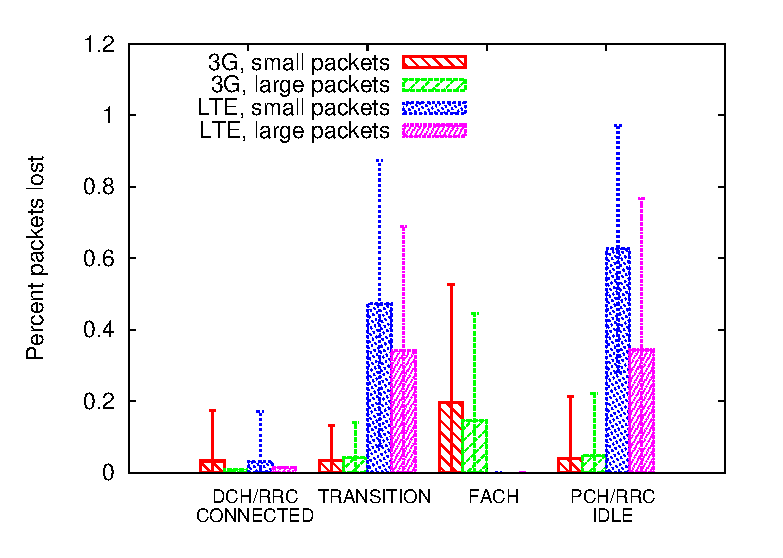
\includegraphics[width=0.45\textwidth]{figs/loss_compare.eps}
\end{center}
\ncaption{Packets lost per state as a percent. Note high losses during transition and RRC\_{}IDLE for LTE.} 
\label{fig:loss_compare}
\end{figure}

Overall, it can be seen that the phenomena we have observed in our controlled experiments on \Paperonly{Carrier C1}\TReport{T-Mobile} devices are of more universal relevance, and more generally that our client-based inference methodology is an effective way to understand trends in RRC state implementations and performance more broadly.   Our inference technique has additionally allowed us to measure the performance characteristics of networks on consumer devices, without requiring any expert knowledge to collect the needed data.



%\mycomment{Tmobile timers consistent.  Only variation is FACH noise for UMTS.  EDGE: timer 1.5s, no FACH-like state.  HSDPA: only one data point, timer 3s, no FACH.  LTE: timer 2s, one data point and kind of noisy (but collecting data on a second data point).  UMTS: 2.5s timer for DCH and another 2.5 on FACH, often eaten by demotion-related delay.}



%\begin{figure}[t!]
%\begin{center}
%
\includegraphics[width=0.45\textwidth]{figs/placeholder.png}
%\end{center}
%\ncaption{Performance for each device for T-Mobile only; colour-code by geographic state - TODO - not much interesting data? lower priority}
%\label{fig:fach_demotion_delay_prevalence}
%\end{figure}
